\chapter{Implementierung}
Der folgende Abschnitt umfasst die praktische Umsetzung dieser Bachelorarbeit. Zunächst werden grundlegende Tools für die Umsetzung der Schnittstelle dargestellt und ihre Anwendung erläutert. Anschließend folgt der Hauptteil dieser Arbeit, die generische Schnittstelle. In dieser werden die Daten für die Evaluation erzeugt und ausgewertet. Einige Probleme sind bei dieser Umsetzung aufgetreten, welche näher beleuchtet werden. Zuletzt werden selbst erstellte CSV Daten präsentiert, die für die generische Schnittstelle von Nöten sind.
\section{Benutzte Tools}
Als Programmierumgebung wurde Jupyter Notebook, eine web-basierte interaktive Umgebung, eingesetzt. Zwei der drei Frameworks (IBM \gls{dp} \& Smartnoise SDK) wurden in der Programmiersprache Python eingesetzt, wodurch in Jupyter Notebook ihre Funktionalität genutzt werden konnten. Nebenbei können durch weitere Python Bibliotheken einfach und schnell Grafiken für die Auswertung der Frameworks realisiert werden. Eine entscheidende Funktionalität dieser Umgebung ist die Unterstützung einer Verbindung zu Servern. Diese verhalf die zeitaufwendigen Berechnungen der Frameworks auf einen Server zu verlagern.

Dagegen wurde das dritte Framework Google \gls{dp} in der Programmiersprache Java umgesetzt, weshalb hierfür die Programmierumgebung Eclipse genutzt wurde. Die Erstellung des Projektes erfolgte durch Bazel, ein Build-Tool zur Automatisierung des Erstellens und Testens von Software. Durch Kommandozeilenbefehle wird der Code erzeugt und durch eine interne Datei von Bazel ausgeführt.

Für die aufwendigen und komplexen Berechnungen innerhalb der aufgerufenen Funktionen des Frameworks wurde ein Server mit den folgenden Systemspezifikationen genutzt: 

Plattform Linux-3.10 64 with-centos-7.9.2009-Core, 18 GB verfügbarer virtueller Arbeitsspeicher, 40 logische Prozessorkerne.

Über eine SSH Verbindung konnten die Berechnungen der Frameworks IBM \gls{dp} und Smartnoise SDK aus dem Jupyter Notebook auf dem Server ausgeführt werden. Dagegen wurde beim Google \gls{dp} das Programm lokal in der Programmierumgebung Eclipse ausgeführt. Zunächst bestand keine Notwendigkeit die Berechnungen auf den Server auszulagern, da die Evaluationsergebnisse schnell berechnet wurden.

\section{Generische Schnittstelle}
In der Datei \textit{source\_data.ipynb} werden die 1,000 generierten Alterswerte erzeugt. Darin wurde der in \cref{sourceData} dargestellte Algorithmus in Python implementiert. Zunächst wird die Verteilung der Wahrscheinlichkeiten für die 19 Altersgruppen in \textit{distribution} vorgegeben. Basierend darauf werden die Gewichte für die zufällige Auswahl des Alters innerhalb einer Altersgruppe festgelegt. Hierfür werden die Wahrscheinlichkeiten gleichermaßen für 100 Alterswerte \textit{weights} verteilt. Somit hat \textit{weights} eine Dimension von 1 Reihen und 100 Spalten. In der Schleife erfolgt 10-mal die Zuweisung von jeweils 100 Werten entsprechend der Gewichtung durch \textit{weights}. Letztendlich befinden sich dann 1000 synthetische Alterswerte in \textit{sourcedata} vor. Davon wird der originale Durchschnitt ohne Verrauschen 1000-mal genommen und in der Datei \textit{originalMean.csv} abgespeichert. Aus den 1000 Alterswerte werden zwei \textit{neighboring datasets} (benachbarte Datensätze) berechnet und in \textit{d1Data.csv} und \textit{d2Data.csv} gespeichert. Diese zwei Datensätze sind für die Berechnung der Metriken nach der Definition von \gls{dp} notwendig, die auf der Aussage von zwei Datensätzen basiert \parencite{Dwork2006}.
\begin{algorithm}[htbp]
	\caption{Erzeugung der 1000 Alterswerte basierend auf der Wahrscheinlichkeitsverteilung von Dezember}\label{sourceData}
	\begin{algorithmic}[1]
		\State $distribution \gets [4,9,10 ... 0.5,0.5]$
		\State $weights \gets [4,4,4,4,4,9,9,9,9,9,10 ... ,0.5,0.5,0.5,0.5,0.5]$
		\For{$i$ $to$ $10$}
		\State $sourceData\gets random.choices(range(0,100),
		weights, k=100)$	
		\EndFor
	\end{algorithmic}
\end{algorithm}

In der Datei \textit{metrics.ipynp} ist das Objekt \textit{Metrics} mit seinen Attributen definiert. Diese sind die Metriken der Evaluation. Ab dem Kaptiel 2.1.5 werden diese nähere erläutert.

In der Datei \textit{dpEvaluator.ipynp} ist die Klasse DPEvaluator definiert. Sie beinhaltet für jede Metrik die benötigte Methode, um sie zu berechnen.

Die bis hier genannten Dateien stellen das Grundgerüst für die Evaluation da. Dieses ist der obere Teil der Gesamtübersicht der generischen Schnittstelle in der \cref{fig:interface_overview}. Zunächst folgt die Generierung der drei CSV Dateien \textit{originalMean.csv, d1Data.csv} und \textit{d2Data.csv} aus der Datei \textit{source\_data.ipynb}. Anschließend können die Frameworks aus diesen den verrauschten Durchschnitt der verschiedenen $\epsilon$-Werte sowie die daraus resultierenden Werte der Metriken berechnen. Ihre Ergebnisse werden in weiteren CSV Dateien gespeichert, sodass sie in der Datei results.ipynb gemeinsam in Diagrammen angezeigt werden können.

Diese Basis wird benötigt, damit die Frameworks den verrauschten Durchschnitt der Alterswerte aus den Dateien \textit{sourcedata.ipynp} berechnen können und von diesen Ergebnissen die Werte der Metriken erhalten.

Nun können die Frameworks ihre \gls{dp} Funktion Durchschnitt darauf anwenden und davon die Metriken berechnen. Dies erfolgt in den Dateien \textit{ibmResults.ipynb}, \textit{snResults,ipynp} und \textit{googleResults.ipynb}.

\begin{figure}[!htbp]
	\centering
	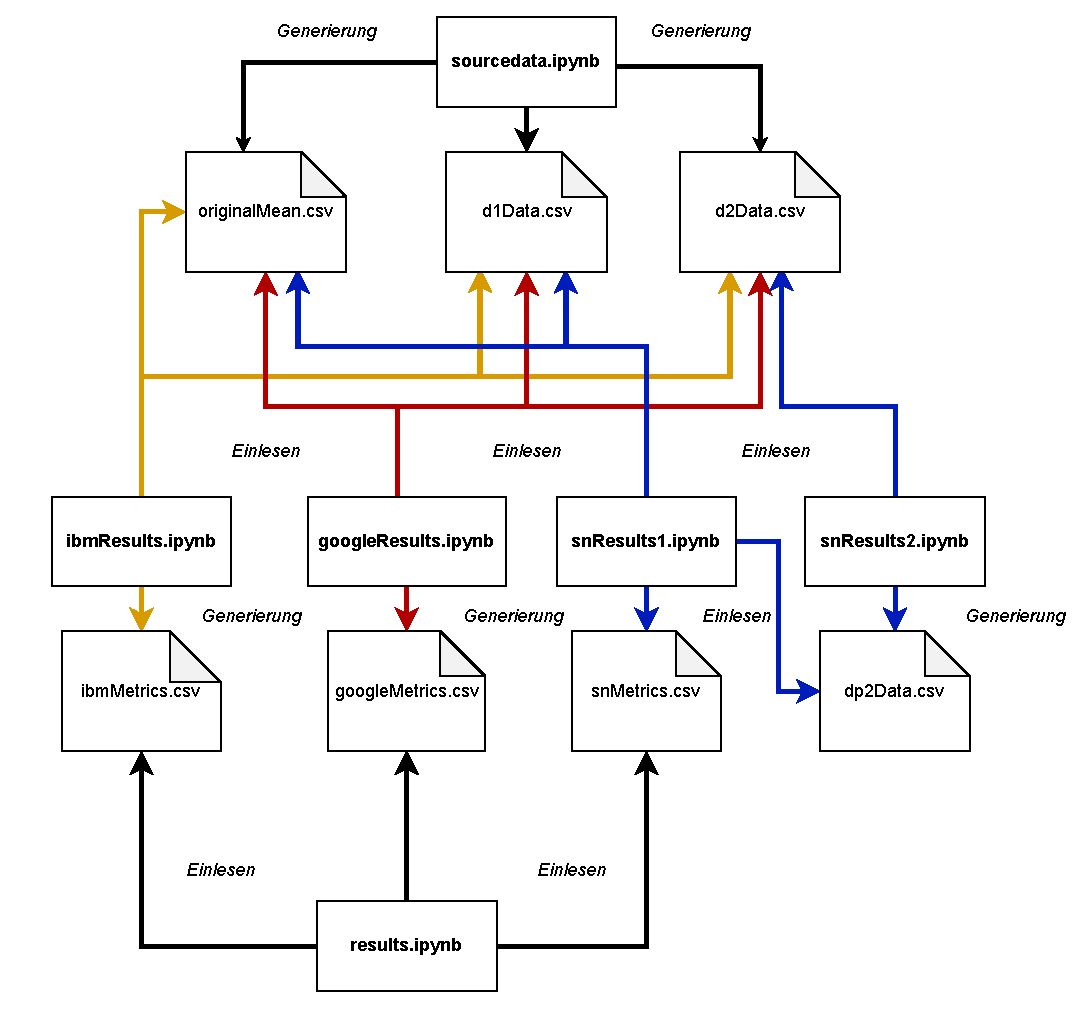
\includegraphics[scale=0.6]{./images/interface_overview.pdf}
	\caption{Eine Übersicht der generischen Schnittstelle für die Evaluation der Frameworks.}
	\label{fig:interface_overview}
\end{figure}

In diesen drei Dateien wird folgender \cref{noisedData} ausgeführt.
Nachdem die drei grundlegenden drei Dateien $d1Data$, $d2Data$ und originalMean gelesen sind, folgt darauf in der verschachtelten \textit{For-Schleife} die Berechnung der verrauschten Durchschnitte entsprechend der verschiedenen $\epsilon$ Werten. Diese sind für die Berechnungen der Metriken in Zeile 10 erforderlich. Jedes Framework berechnet ihre eigenen Metriken für die $\epsilon$-Werte und speichert sie in ihrer CSV-Datei ab. Bei dem Framework Smartnoise SDK liegt eine Besonderheit vor, da es zwei Dateien \textit{snResults1.ipynb} und \textit{snResults2.ipynb} verwendet. Hierbei wird lediglich die Berechnung der verrauschten Werte in Zeile 6 und 7 separiert in diesen Dateien berechnet. Somit kann die Berechnung parallel ausgeführt werden, da sonst die Laufzeit erheblich höher ist. Semantisch entsprechen sie gemeinsam dem Code in Zeile 1 bis 10.
\begin{algorithm}[t]
	\caption{Die Erzeugung der verrauschten Durchschnittswerte und die Berechnung aus ihnen resultierenden metrischen Werten}\label{noisedData}
	\begin{algorithmic}[1]
		\State $d1Data\gets read(d1Data.csv)$
		\State $d2Data\gets read(d2Data.csv)$
		\State $originalMean\gets read(originalMean.csv)$
		\For{$e$ $in$ $epsilons$}
		\For{$index=0$ $to$ $1000$}
		\State $noisedMean1\gets  dp.mean(d1Data)$
		\State $noisedMean2\gets  dp.mean(d2Data)$
		\EndFor
		\EndFor
		\State $metrics\gets calculateMetrics(noisedMean1,noisedMean2,originalMean)$
	\end{algorithmic}
\end{algorithm}
In der letzten Datei results.ipynb erfolgt lediglich die Veranschaulichung der Metriken gemeinsam in einem Diagramm. 

\section{Datenstruktur}
Für die Evaluation werden bestimmte Daten in CSV Dateien abgespeichert, damit die generische Schnittstelle flexibel und unabhängig von den Frameworks funktionieren kann.

Die drei CSV Dateien $d1Data$, $d2Data$ und $originalMean$ dienen als Grundbasis der Evaluation. Wenn diese neu berechnet werden, muss die gesamte Evaluation für einen Vergleich erneut durchgeführt werden. Damit dies nicht jedes Mal vom neuen erforderlich ist, werden sie einmal abgespeichert und von den Frameworks nur gelesen.

Die weitere Separierung der Frameworks in eigene Jupyter Notebooks und ihre Abspeicherung der Ergebnisse in CSV Dateien soll die Flexibilität unterstützen. Es können beliebig viele Durchläufe der \gls{dp} Berechnungen erfolgen, welche in den entsprechenden results.csv gespeichert werden (siehe \cref{fig:interface_overview}). In der Datei \textit{results.ipynb} werden alle Durchläufe zu jedem Framework in einem Array gespeichert. Je nach Auswahl des Arrayfeldes für ein bestimmtes Framework kann ein spezifischer Durchlauf veranschaulicht werden. Dies erleichtert den Vergleich der Werte aus den Metriken.

\section{Probleme}
Eine große Herausforderung dieser Arbeit war es geeignete Metriken für die Evaluation zu finden. Trotz intensiver Literaturrecherche bezüglich Papers im Bereich \gls{dp} wurden keine vergleichsweise Evaluationen wie diese gefunden. Nach genauerem Lesen wurden ein paar Papers im Bereich Analyse von \gls{dp} gefunden, die sich mit der Genauigkeit sowie Privatsphäre von \gls{dp} beschäftigten. Jedoch gab es keine expliziten in Bezug auf Frameworks. Nach langer Recherche wurde im Framework Smartnoise SDK eine Teilbibliothek gefunden, welche sich für Evaluation von \gls{dp} Algorithmen sich eignet \parencite{SNEVAL}. Hierbei werden 8 Metriken für die Evaluation eingesetzt. Diese wurden analysiert und beurteilt, ob sie für diese Bachelorarbeit sinnvoll und nutzbar sind. Dabei wurde bei Fachliteraturen in der Mathematik recherchiert und in Tests in Python auf Tauglichkeit überprüft. Davon wurden 5 Metriken übernommen.

In weiteren verschiedenen Veröffentlichungen wurde zur Bestimmung der Genauigkeit das Modell einer logistischen Regression verwendet. Diese galt als eine Möglichkeit die Auswirkung des Verrauschens auf Rohdaten zu beurteilen. Für diese Bachelorarbeit wurde ebenfalls dieses Modell in Python implementiert und veranschaulicht. Nach einigen Tests sowie Recherche folgte, dass das Szenario dieser Bachelorarbeit für dieses Modell zu einfach ist. Dies lag am Kriterium, welcher der originale Durchschnitt war. Das Modell konnte schnell dieses Kriterium lernen. Somit wurde eine Genauigkeit (score) von ca. 98\% stets erreicht. Aufgrund dessen hat die Aussagekraft für eine Beurteilung des Verrauschens gefehlt. Schließlich wurde dieses Modell für diese Arbeit nicht miteingebracht.

Eine große Hürde war die Feststellung der Gründe für die entgegen den Erwartungen auftretenden Ergebnisse. Die Frameworks beinhalten bekannte Mechanismen wie Laplace und weitere. Jedoch ist die Prozedur des Frameworks intern nicht von außen nachvollziehbar. Das Verrauschen folgt einem Mechanismus, welcher unterschiedlich implementiert werden kann. Um die Ergebnisse auf Richtigkeit und Gültigkeit zu prüfen, wurden neben den Ergebnissen auch Zwischenergebnisse der Berechnungen gespeichert. Diese halfen die Berechnungen der Frameworks besser nachzuvollziehen. Des Weiteren folgten in den Ergebnissen der Metriken Abweichungen aufgrund von kleinen $\epsilon$-Werten. Eine valide Beurteilung der Leistung des Frameworks wäre somit nicht möglich gewesen. Insgesamt konnte ein geeignetes Intervall an $\epsilon$-Werten sowie plausible Ergebnisse bestimmt werden. 